\documentclass{beamer}
\usepackage{../mysty}

\title{Week 08: Connectivity}
\author{FanFly}
\date{April 26, 2020}

\begin{document}

\begin{frame}
  \titlepage
\end{frame}

\section{Data Structures}
\subsection{Common Data Structures}
\begin{frame}{Data Structures}
  Let us review some data structures we have learned. \pause
  \begin{block}{List}
    \pause
    \begin{itemize}
      \item Create: $O(1)$ time (amortized). \pause
      \item Search: $O(n)$ time. \pause
      \item Update: $O(1)$ time. \pause
      \item Delete: $O(n)$ time.
    \end{itemize}
  \end{block}
  \pause
  \begin{block}{Dictionary / Set}
    \begin{itemize}
      \pause
      \item Create: $O(1)$ time (average-case). \pause
      \item Search: $O(1)$ time (average-case). \pause
      \item Update: $O(1)$ time. \pause
      \item Delete: $O(1)$ time.
    \end{itemize}
  \end{block}
\end{frame}

\subsection{Data Structures for Graphs}
\begin{frame}{Data Structures for Graphs}
  We learned adjacency lists and adjacency matrix last week.
  \begin{block}{Adjacency List}
    \pause
    \begin{itemize}
      \item Preprocess: $O(n + m)$ time. \pause
      \item Check if vertices $u$ and $v$ are adjacent: $O(d(u))$ time.
    \end{itemize}
  \end{block}
  \pause
  \begin{block}{Adjacency Matrix}
    \pause
    \begin{itemize}
      \item Preprocess: $O(n^2)$ time. \pause
      \item Check if vertices $u$ and $v$ are adjacent: $O(1)$ time.
    \end{itemize}
  \end{block}
\end{frame}

\section{Connectivity}
\subsection{Connectivity}
\begin{frame}{Connectivity}
  In a graph $G = (V, E)$, vertices $u$ and $v$ are said to be \emph{connected}
  if there is a path from $u$ to $v$. \pause
  \begin{itemize}
    \item Also, we say that a graph is \emph{connected} if any two vertices in
    the graph are connected. \pause
  \end{itemize}
  \vspace{1em}
  Today, we want to build a data structure satisfying the following properties.
  \pause
  \begin{block}{A Mysterious Data Structure}
    \pause
    \begin{itemize}
      \item Preprocess: $O(n + m)$ time. \pause
      \item Check if vertices $u$ and $v$ are {\color{red} connected}:
      $O(1)$ time.
    \end{itemize}
  \end{block}
\end{frame}

\subsection{Connected Components}
\begin{frame}{Connected Components}
  We want to label the vertices with the \emph{connected components} they
  belong to. \pause
  \begin{itemize}
    \item A connected component of a graph is a maximal set of vertices such
    that each pair of vertices are connected.
  \end{itemize}
  \vspace{1em}
  \pause
  \begin{figure}
    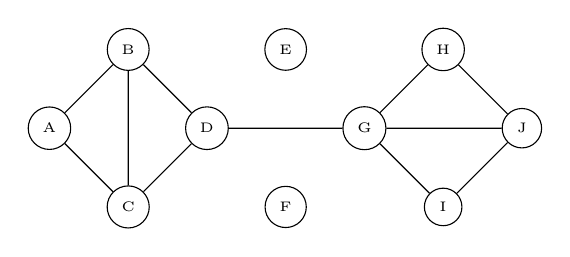
\begin{tikzpicture}
      \begin{scope}[every node/.style={circle,draw,font=\tiny}]
        \node (A) at (-3, 0) {A};
        \node (B) at (-2, 1) {B};
        \node (C) at (-2, -1) {C};
        \node (D) at (-1, 0) {D};
        \node (E) at (0, 1) {E};
        \node (F) at (0, -1) {F};
        \node (G) at (1, 0) {G};
        \node (H) at (2, 1) {H};
        \node (I) at (2, -1) {I};
        \node (J) at (3, 0) {J};
      \end{scope}
      \begin{scope}[every node/.style={font=\scriptsize}]
        \draw (B) -- (A) -- (C) -- (D) -- (B) -- (C);
        \draw (D) -- (G) -- (H) -- (J) -- (I) -- (G) -- (J);
      \end{scope}
    \end{tikzpicture}
  \end{figure}
\end{frame}

\begin{frame}{Connected Components (cont.)}
  For each connected components, we choose a representative to identify it.
  \vspace{1.5em}
  \begin{figure}
    \begin{tikzpicture}
      \begin{scope}[every node/.style={circle,draw,font=\tiny}]
        \node[fill=CustomRed!80] (A) at (-3, 0) {A};
        \node[fill=CustomRed!20] (B) at (-2, 1) {B};
        \node[fill=CustomRed!20] (C) at (-2, -1) {C};
        \node[fill=CustomRed!20] (D) at (-1, 0) {D};
        \node[fill=CustomBlue!80] (E) at (0, 1) {E};
        \node[fill=CustomGreen!80] (F) at (0, -1) {F};
        \node[fill=CustomRed!20] (G) at (1, 0) {G};
        \node[fill=CustomRed!20] (H) at (2, 1) {H};
        \node[fill=CustomRed!20] (I) at (2, -1) {I};
        \node[fill=CustomRed!20] (J) at (3, 0) {J};
      \end{scope}
      \begin{scope}[every node/.style={font=\scriptsize}]
        \draw (B) -- (A) -- (C) -- (D) -- (B) -- (C);
        \draw (D) -- (G) -- (H) -- (J) -- (I) -- (G) -- (J);
      \end{scope}
    \end{tikzpicture}
  \end{figure}
\end{frame}

\section{Depth-First Search}
\subsection{Representing a Graph}
\begin{frame}[fragile]{The Graph Class}
  We are going to introduce a very useful ``algorithm'', which is called
  \emph{depth-first search}. \pause \\[1em]
  First we construct a class in Python called \lstinline{Graph}. \pause
  \begin{block}{}
    \scriptsize
    \begin{lstlisting}[gobble=4]
    class Graph:
    \end{lstlisting}
    \pause
    \begin{lstlisting}[gobble=4]
        def __init__(self, vertices):
            self.vertices = list(vertices)
            self.adj = {u: [] for u in vertices}
    \end{lstlisting}
    \pause
    \begin{lstlisting}[gobble=4]

        def add_edge(self, u, v):
            self.adj[u].append(v)
            self.adj[v].append(u)
    \end{lstlisting}
  \end{block}
\end{frame}

\begin{frame}[fragile]{The Graph Class (cont.)}
  For example, we can represent the graph as follows. \pause
  \begin{figure}
    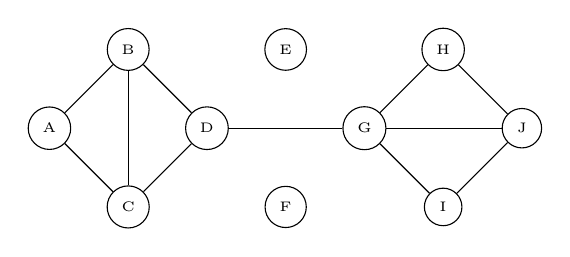
\begin{tikzpicture}
      \begin{scope}[every node/.style={circle,draw,font=\tiny}]
        \node (A) at (-3, 0) {A};
        \node (B) at (-2, 1) {B};
        \node (C) at (-2, -1) {C};
        \node (D) at (-1, 0) {D};
        \node (E) at (0, 1) {E};
        \node (F) at (0, -1) {F};
        \node (G) at (1, 0) {G};
        \node (H) at (2, 1) {H};
        \node (I) at (2, -1) {I};
        \node (J) at (3, 0) {J};
      \end{scope}
      \begin{scope}[every node/.style={font=\scriptsize}]
        \draw<3-> (A) -- (B);
        \draw<4-> (A) -- (C);
        \draw<5-> (B) -- (C);
        \draw<6-> (B) -- (D);
        \draw<7-> (C) -- (D);
        \draw<8-> (D) -- (G);
        \draw<9-> (G) -- (H);
        \draw<10-> (G) -- (I);
        \draw<11-> (G) -- (J);
        \draw<12-> (H) -- (J);
        \draw<13-> (I) -- (J);
      \end{scope}
    \end{tikzpicture}
  \end{figure}
  \begin{block}{}
    \tiny
    \begin{lstlisting}[gobble=4]
    >>> G = Graph(["A", "B", "C", "D", "E", "F", "G", "H", "I", "J"])
    \end{lstlisting}
    \pause
    \begin{lstlisting}[gobble=4]
    >>> G.add_edge("A", "B")
    \end{lstlisting}
    \pause
    \begin{lstlisting}[gobble=4]
    >>> G.add_edge("A", "C")
    \end{lstlisting}
    \pause
    \begin{lstlisting}[gobble=4]
    >>> G.add_edge("B", "C")
    \end{lstlisting}
    \pause
    \begin{lstlisting}[gobble=4]
    >>> G.add_edge("B", "D")
    \end{lstlisting}
    \pause
    \begin{lstlisting}[gobble=4]
    >>> G.add_edge("C", "D")
    \end{lstlisting}
    \pause
    \begin{lstlisting}[gobble=4]
    >>> G.add_edge("D", "G")
    \end{lstlisting}
    \pause
    \begin{lstlisting}[gobble=4]
    >>> G.add_edge("G", "H")
    \end{lstlisting}
    \pause
    \begin{lstlisting}[gobble=4]
    >>> G.add_edge("G", "I")
    \end{lstlisting}
    \pause
    \begin{lstlisting}[gobble=4]
    >>> G.add_edge("G", "J")
    \end{lstlisting}
    \pause
    \begin{lstlisting}[gobble=4]
    >>> G.add_edge("H", "J")
    \end{lstlisting}
    \pause
    \begin{lstlisting}[gobble=4]
    >>> G.add_edge("I", "J")
    \end{lstlisting}
  \end{block}
\end{frame}

\subsection{Algorithm}
\begin{frame}[fragile]{Depth-First Search}
  Now we introduce the depth-first search algorithm. \pause
  \begin{block}{}
    \scriptsize
    \begin{lstlisting}[gobble=4]
    class Graph:
        ...
        def dfs(self):
            visited = set()
    \end{lstlisting}
    \pause
    \begin{lstlisting}[gobble=4]
            # A recursive function used by depth first search
            def dfs_visit(u):
                visited.add(u)
                for v in self.adj[u]:
                    if v not in visited:
                        dfs_visit(v)
    \end{lstlisting}
    \pause
    \begin{lstlisting}[gobble=4]
            # Start depth first search
            for u in self.vertices:
                if u not in visited:
                    dfs_visit(u)
    \end{lstlisting}
  \end{block}
  \pause
  In fact, the method \lstinline{dfs()} does not do anything, but it traverses
  all the vertices exactly once in a specific order.
\end{frame}

\begin{frame}[fragile]{Depth-First Search (cont.)}
  \begin{block}{}
    \tiny
    \begin{lstlisting}[gobble=4,stringstyle=\color{black}]
    >>> for u in G.vertices:
    ...     print(u, G.adj[u])
    ... 
    A ["B", "C"]
    B ["A", "C", "D"]
    C ["A", "B", "D"]
    D ["B", "C", "G"]
    E []
    F []
    G ["D", "H", "I", "J"]
    H ["G", "J"]
    I ["G", "J"]
    J ["G", "H", "I"]
    \end{lstlisting}
  \end{block}
  \begin{figure}
    \begin{tikzpicture}
      \begin{scope}[every node/.style={circle,draw,font=\tiny}]
        \node<1> (A) at (-3, 0) {A};
        \node<2->[fill=CustomYellow!30] (A) at (-3, 0) {A};
        \node<-2> (B) at (-2, 1) {B};
        \node<3->[fill=CustomYellow!30] (B) at (-2, 1) {B};
        \node<-3> (C) at (-2, -1) {C};
        \node<4->[fill=CustomYellow!30] (C) at (-2, -1) {C};
        \node<-4> (D) at (-1, 0) {D};
        \node<5->[fill=CustomYellow!30] (D) at (-1, 0) {D};
        \node<-5> (G) at (1, 0) {G};
        \node<6->[fill=CustomYellow!30] (G) at (1, 0) {G};
        \node<-6> (H) at (2, 1) {H};
        \node<7->[fill=CustomYellow!30] (H) at (2, 1) {H};
        \node<-7> (J) at (3, 0) {J};
        \node<8->[fill=CustomYellow!30] (J) at (3, 0) {J};
        \node<-8> (I) at (2, -1) {I};
        \node<9->[fill=CustomYellow!30] (I) at (2, -1) {I};
        \node<-9> (E) at (0, 1) {E};
        \node<10->[fill=CustomYellow!30] (E) at (0, 1) {E};
        \node<-10> (F) at (0, -1) {F};
        \node<11>[fill=CustomYellow!30] (F) at (0, -1) {F};
      \end{scope}
      \begin{scope}[every node/.style={font=\scriptsize}]
        \draw (A) -- (B);
        \draw (A) -- (C);
        \draw (B) -- (C);
        \draw (B) -- (D);
        \draw (C) -- (D);
        \draw (D) -- (G);
        \draw (G) -- (H);
        \draw (G) -- (I);
        \draw (G) -- (J);
        \draw (H) -- (J);
        \draw (I) -- (J);
      \end{scope}
    \end{tikzpicture}
  \end{figure}
\end{frame}

\subsection{Time Complexity}
\begin{frame}[fragile]{Time Complexity of Depth-First Search}
  \begin{block}{}
    \tiny
    \begin{lstlisting}[gobble=4]
    class Graph:
        ...
        def dfs(self):
            visited = set()
            # A recursive function used by depth first search
            def dfs_visit(u):
                visited.add(u)
                for v in self.adj[u]:
                    if v not in visited:
                        dfs_visit(v)
            # Start depth first search
            for u in self.vertices:
                if u not in visited:
                    dfs_visit(u)
    \end{lstlisting}
  \end{block}
  What is the time complexity of depth-first search? \pause
  \begin{itemize}
    \item The function \lstinline{dfs_visit()} is called exactly once for each
    vertex. \pause
    \item During the execution of \lstinline{dfs_visit()} for vertex $u$, the
    \lstinline{for} loop runs in $\Theta(d(u))$ time. \pause
    \item Thus, the overall running time is $\Theta(n + m)$.
  \end{itemize}
\end{frame}

\subsection{Using DFS To Find Connected Components}
\begin{frame}{Finding Connected Components}
  Depth-first search can be used to find connected components. \pause
  \begin{itemize}
    \item When \lstinline{dfs()} calls \lstinline{dfs_visit()}, a connected
    component is found. \pause
    \item Thus, with little revision we can use \lstinline{dfs()} to label
    the vertices with the connected component they belong to.
  \end{itemize}
\end{frame}

\begin{frame}[fragile]{Finding Connected Components (cont.)}
  We use a dictionary \lstinline{label} to store the representative of the
  connected component that a vertex belongs to.
  \begin{block}{}
    \scriptsize
    \begin{lstlisting}[gobble=4]
    class Graph:
        ...
        def dfs(self):
          visited = set()
          label = {}
          # A recursive function used by depth first search
          def dfs_visit(u, r):
              label[u] = r
              visited.add(u)
              for v in self.adj[u]:
                  if v not in visited:
                      dfs_visit(v, r)
          # Start depth first search
          for u in self.vertices:
              if u not in visited:
                  dfs_visit(u, u)
          return label
    \end{lstlisting}
  \end{block}
\end{frame}

\begin{frame}[fragile]{Finding Connected Components (cont.)}
  \begin{block}{}
    \tiny
    \begin{lstlisting}[gobble=4]
    >>> label = G.dfs()
    >>> for u in G.vertices:
    ...     print(u, label[u])
    ... 
    A A
    B A
    C A
    D A
    E E
    F F
    G A
    H A
    I A
    J A
    \end{lstlisting}
  \end{block}
  \begin{figure}
    \begin{tikzpicture}
      \begin{scope}[every node/.style={circle,draw,font=\tiny}]
        \node[fill=CustomRed!80] (A) at (-3, 0) {A};
        \node[fill=CustomRed!20] (B) at (-2, 1) {B};
        \node[fill=CustomRed!20] (C) at (-2, -1) {C};
        \node[fill=CustomRed!20] (D) at (-1, 0) {D};
        \node[fill=CustomBlue!80] (E) at (0, 1) {E};
        \node[fill=CustomGreen!80] (F) at (0, -1) {F};
        \node[fill=CustomRed!20] (G) at (1, 0) {G};
        \node[fill=CustomRed!20] (H) at (2, 1) {H};
        \node[fill=CustomRed!20] (I) at (2, -1) {I};
        \node[fill=CustomRed!20] (J) at (3, 0) {J};
      \end{scope}
      \begin{scope}[every node/.style={font=\scriptsize}]
        \draw (B) -- (A) -- (C) -- (D) -- (B) -- (C);
        \draw (D) -- (G) -- (H) -- (J) -- (I) -- (G) -- (J);
      \end{scope}
    \end{tikzpicture}
  \end{figure}
\end{frame}

\begin{frame}{Conclusion}
  With depth-first search we can know the connected component a vertex belongs
  to, and thus we have the following data structure. \pause
  \begin{block}{Adjacency List with Label}
    \begin{itemize}
      \item Preprocess: $O(n + m)$ time.
      \item Check if $u$ and $v$ are {\color{red} connected}: $O(1)$ time.
    \end{itemize}
  \end{block}
\end{frame}

\subsection{Iterative Method}
\begin{frame}[fragile]{Iterative Method}
  In fact, we can use a \emph{stack} to eliminate recursion! \pause
  \begin{block}{}
    \scriptsize
    \begin{lstlisting}[gobble=4]
    class Graph:
        ...
        def dfs(self):
            visited = set()
            # A non-recursive function used by depth first search
            def dfs_visit(u):
                stack = [u]
                while stack:
                    u = stack.pop()
                    if u not in visited:
                        visited.add(u)
                        for v in self.adj[u]:
                            stack.append(v)
            # Start depth first search
            for u in self.vertices:
                if u not in visited:
                    dfs_visit(u)
    \end{lstlisting}
  \end{block}
\end{frame}

\section{Exercises}
\subsection{\#1}
\begin{frame}{Exercise \#1}
  Consider the following problem. \pause
  \begin{block}{Connected Component Problem}
    \begin{itemize}
      \item Input: A graph $G$ with $n$ vertices and $m$ edges.
      \item Output: The number of connected components of $G$.
    \end{itemize}
  \end{block}
  \pause
  What is the time complexity of the connected component problem?
  \begin{multicols}{2}
    \begin{itemize}
      \item $\Theta(n + m)$
      \item $\Theta(n^2)$
      \item $\Theta((n + m)\log n)$
      \item $\Theta(2^n)$ \pause
    \end{itemize}
  \end{multicols}
  \begin{block}{Solution}
    An $O(n + m)$-time depth-first search can solve the connected component
    problem.
    Thus, its time complexity is $\Theta(n + m)$ since the input size is
    $\Omega(n + m)$.
  \end{block}
\end{frame}

\subsection{\#2}
\begin{frame}{Exercise \#2}
  Let $G = (V, E)$ with $n$ vertices and $m$ edges.
  Let $u, v, w$ be vertices in $G$. \pause \\
  Which of the following statements is true? \pause
  \begin{itemize}
    \item A vertex can have at most $n$ neighbors. \pause
    \item $m$ should not be less than $n$. \pause
    \item If $u$ and $v$ are adjacent and $v$ and $w$ are adjacent, then
    $u$ and $w$ are adjacent. \pause
    \item If $u$ and $v$ are connected and $v$ and $w$ are connected, then
    $u$ and $w$ are connected. \pause
  \end{itemize}
  \begin{block}{Solution}
    Only the last statement is correct.
  \end{block}
\end{frame}

\subsection{\#3}
\begin{frame}{Exercise \#3}
  Let $G = (V, E)$ with $|V| = n$ and $|E| = m$. \pause
  Furthermore, let $A$ and $C$ be $n \times n$ matrices such that
  \begin{equation*}
    A_{ij} =
    \begin{cases}
      1, & \text{if $v_i$ and $v_j$ are adjacent} \\
      0, & \text{otherwise}
    \end{cases}
  \end{equation*}
  and
  \begin{equation*}
    C_{ij} =
    \begin{cases}
      1, & \text{if $v_i$ and $v_j$ are connected} \\
      0, & \text{otherwise}.
    \end{cases}
  \end{equation*}
  \pause
  Let $B = I + A + A^2 + \cdots + A^{n-2} + A^{n-1}$. \\
  What is the relation between $B$ and $C$? \pause
  \begin{block}{Solution}
    $C_{ij} = 1$ if and only if $B_{ij} \geq 1$.
  \end{block}
\end{frame}

\end{document}